\documentclass[11pt]{article}

% Language setting
% Replace `english' with e.g. `spanish' to change the document language
\usepackage[english]{babel}

% Set page size and margins
% Replace `letterpaper' with `a4paper' for UK/EU standard size
\usepackage[a4paper,top=1.75cm,bottom=1.75cm,left=1.5cm,right=1.5cm,marginparwidth=1.75cm]{geometry}

% Useful packages
\usepackage{amsmath,amssymb,amsfonts,multicol}
\usepackage{graphicx}
\usepackage{caption}
\usepackage[colorlinks=true, allcolors=blue]{hyperref}
\newenvironment{Figure}
  {\par\medskip\noindent\minipage{\linewidth}}
  {\endminipage\par\medskip}

\title{\textsf{\textbf{f}}}
\author{Antoine GISSLER}
\date{January 10th, 2023}

\begin{document}
\noindent\huge\textbf{\textsf{Generation of optimized structures using Particle Swarn Optimization (PSO)}}\normalsize\vspace{1em}\\
\large \textsf{Antoine GISSLER -- Sorbonne Université}
\begin{multicols}{2}
\section*{Introduction}

For as long as both theoretical and technological progress entitled scientists to do, there has been a wide interest to understand the nanoscopic scale of matter. Indeed, doing so makes it possible to understand the processes of transition and their results when matter is subject to changing conditions, such as pressure or temperature. Indeed, it has been observed that applying new conditions could alter various variables in matter: in the case of water ices, the symmetry and the number of H-bonds that are possible can be altered by the variation of pressure. Moreover, these changes can lead to variation of properties of materials, which could lead to serious issues in fields where they have expected to withstand critical infrastructure (aeronautics, nuclear powerplants, etc...). Yet, a full understanding of every material is hard to achieve: even for very common elements such as water, there is still today space for discussion over some of its solid phases \cite{Hansen2021-bk}.

Up to recently, crystalline structure for materials was obtained (or at least helped by it) through experimental studies: X-Ray diffraction (XRD) being almost the norm in order to characterize anything in Material Science. However, this implies that the crystallized experimental structure shall be accessible, which requires consequent setups in the case of extreme conditions being studied. In the case of a complete theoretical study through numerical calculations, it implies to find the global minimum of the potential energy surface of the molecule, which depends of many parameters (for a molecule containing $N$ atoms, it can go up to $3N-3$ degrees of freedom, including bond length, angles of rotation and torsion). Yet, as simple as the concept may seem, it hides a very complex truth: finding the global minimum of a ensemble containing many parameters, is not an easy task at all. Without any hint on initial configurations to begin optimization with, simulations can get stuck in local minima. Moreover, finding this minimum in the case of a crystalline phase is also conditionned to the right selection for the symmetry of the crystal: yet again increasing the complexity.\vspace{1em}

\noindent The quest for finding global minima in the case of molecular systems has been done through various approaches (a visual presentation is available in Figure 1):
\begin{itemize}
    \itemsep0em
    \item \textbf{Monte Carlo:} involves random changes on parameters and accept the modification using probabilistic techniques \cite{PhysRevB.95.144104}
    \item \textbf{Simulated annealing:} the temperature of the system is increased so that every configuration is accessible, and then is slowly decreased for the system to converge to the global minimum in a Monte-Carlo fashion
    \item \textbf{Minima hopping:} perturbates the configuration at local minimum to explore nearbies ; if new configuration has lower energy, configuration is updated ; if not the perturbation module is increased
    \item \textbf{Basin hopping:} similar to minima hopping, but focuses rather on the basins of potential energy
    \item \textbf{Metadynamics:} enhances the sampling of rare events, and thus permits a quasi-total sampling of the potential energy surface (PES) ; in this case the global minimum can be easily found
    \item \textbf{Genetic algorithm:} inspired by the principles of evolution of living species, theses algorithm induce selection, mutation, and recombination to optimized configurations
\end{itemize}
\bigskip

              \noindent 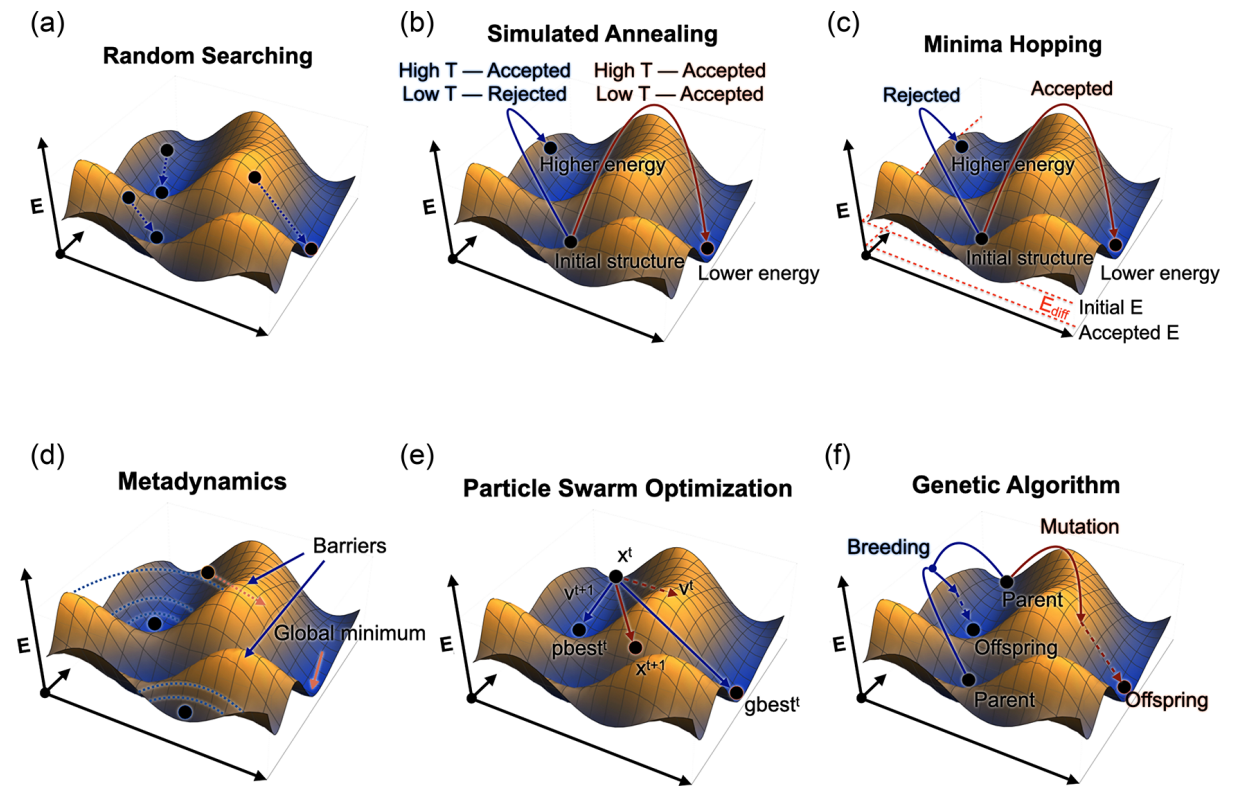
\includegraphics[width=\columnwidth]{figures/optim_figures.png}
                \captionof{figure}{Schematic explanation of various crystal structure prediction methods, by Falls et al. \cite{Falls2020}}\medskip

Each method has its own advantages and inconvenients, and has been probed for the generation of configurations. Thus, there is still no consensus for a specific method, as techniques can be better in some cases. \vspace{1em}

This report, based on the publication from Naden Robinson et al. \cite{original}, tackles the application of another generalized optimization algorithm (Particle Swarn Optimization) for the purposes of potential energy surfaces exploration and the determination of the optimized geometry for extreme conditions. The study is based on the exploration of ammonia-water mixtures present inside planets of our solar system (especially Uranus and Neptune). In these mantles, there exists some particularly harsh conditions, that are not existing in our planet: indeed, high temperatures and pressure can be reached; thus accessing zones of the phase diagram of this mixture that were never explored previously. Furthermore, it is almost impossible in this case to use experiments in the first place to have first guesses, and as we have no clue about any stoechiometry, symmetry or parameters, sampling the entire potential energy surface would be very computationally expensive. Those reasons also exclude many of the above methods, that would require an initial configuration, and/or a clear final destination. As a matter of consequence, using a smart optimization technique is, of course, of high importance.

\section*{Particle Swarn Optimization}
\subsection*{Theoretical background}
Particle Swarm Optimization (also called PSO) is a population-based optimization algorithm that simulates the social behavior of birds or insects, such as flocking or swarming. Every iteration, one optimization simulation's (called a particle) trajectory is inspired by its own personal local minimum (\verb+pbest+) that it can reach through gradient descent, and the global (on all particle) minimum (\verb+gbest+). Its application for structure discovery was introduced by Wang et al. \cite{PhysRevB.82.094116}, and transcribed into a software (called \textsc{calypso}) by the same authors \cite{WANG20122063}. The particle swarn optimization presents a simple algorithm:
\begin{itemize}
\itemsep0em
    \item Generation of one random structure per symmetry (avoids unnecessary calculations)
    \item Local optimization of every structure
    \item Exclusion of similar structures (through bond characterization matrix)
    \item Generation of new structures by PSO, using personal and flock's histories (see below)
    \item Repeating steps 2, 3 and 4 until convergence is reached
    \item Returns the configuration with the lowest energy
\end{itemize}
The calculation of new structures by PSO formulas is carried out for each parameter individually.
For the $i^\text{th}$ particle, we have the following equation for the calculation of the updated coordinates for dimension $j$:
\begin{equation}
    x_{i,j}^{t+1}=x_{i,j}^{t}+v_{i,j}^{t+1}
\end{equation}
With $v_{i,j}^{t+1}$ its velocity for the $j^\text{th}$ dimension:
\begin{equation}
    v_{i,j}^{t+1}=\omega v_{i,j}^t+c_1r_1(\verb+pbest+_{i,j}^t-x_{i,j}^t)+c_2r_2(\verb+gbest+_{i,j}^t-x_{i,j}^t)
\end{equation}
With $\omega$ being the inertia weight (translating the importance or not of previous velocity), $c_1$ and $c_2$ being respectively the self-confidence and the swarm confidence factor, and $r_i$ being random parameters. By changing the fixed parameters (by fixing them at first, or making them evoluate throughout the simulaton), it is possible to go from global jump, with long hoppings, to a precise localization of the minimum in its basin.
A schematic of an iteration of generation of new coordinates for a particle on a specific coordinate is shown in Figure 2. 
\bigskip

              \noindent 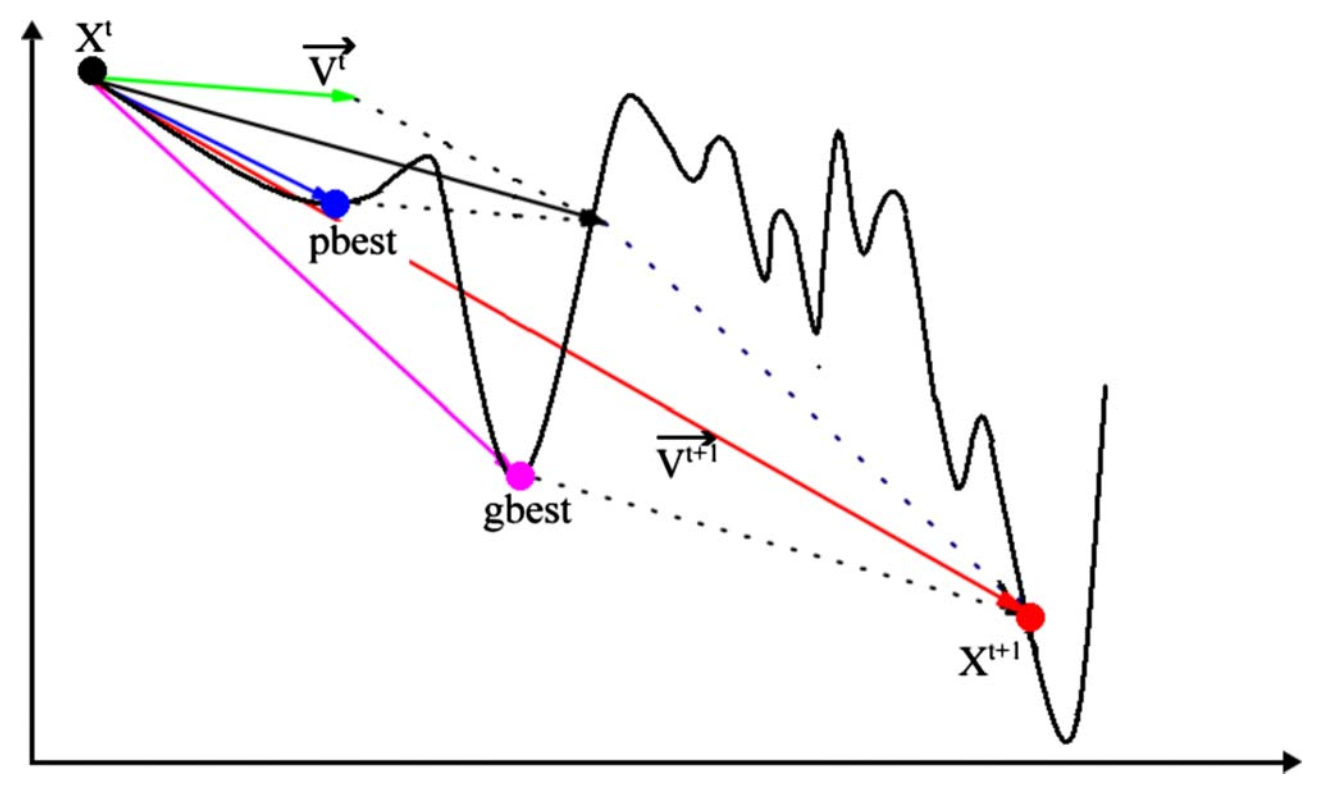
\includegraphics[width=\columnwidth]{figures/PSO.png}
                \captionof{figure}{Schematic explanation of particle swarn optimization on one parameter, by Wang et al. \cite{PhysRevB.82.094116}}\medskip
The advantage of such method is thus clearly visible: by taking into account samplings at various zones of the PES, and forcing particles to travel to a zone of interest, it is possible to force particles to get out of their local minima from one hand, but also to provide a better sampling around zones of interest (some will go further, some before the global minimum found at an iteration, which may lead to the discovery of a better minimum, etc...).\vspace{1em}

Authors announce very interesting results in both their introduction article and the presentation of \textsc{calypso} \cite{PhysRevB.82.094116,WANG20122063}: starting from scratch, and using either DFT or empirical potentials (using the GULP code), it was possible to obtain optimized structures with less than 10 PSO generations (representing around 300 structures).
\subsection*{Programming PSO, trial over a simple two-dimensional study case}
The code that has been developped following the above instructions, is available on Github (\href{https://github.com/antoinegslr/ParticleSwarnOptimization}{link here}). The algorithm was applied on a similar case study (yet with a lower dimensionality for the sake of simplicity): the Eggholder trial function.
\begin{multline*}
    f(x,y)=-(y+47)\sin\left(\sqrt{\left|\frac{x}{2}+(y+47)\right|}\right)\\-x\sin\left(\sqrt{\left|\frac{x}{2}-(y+47)\right|}\right)
\end{multline*}
As it would be in the case of our molecular systems, the function surface is full of hills and wells, with very steep walls in between them. In the case of conventional sampling methods, it would be either very long to sample (hitting only a few units of $x$ away from a minimum gives very different results), or quite easy to get stuck in local minima.\\
In this example, particles were randomly placed (following a uniform distribution) in an initial area: $(x,y)\in\left[-512,512\right]^2$ and were affected random velocities along each dimension ($|v_i|<50$). In order to converge quickly, $\omega$ was set at 0.6 at the beginning, and linearly decreased to 0.3 until the end of the loop; $c_1$ and $c_2$ were equally defined to 1 (equal confidence).\\
As told previously, the particles quickly adopt a similar behavior to a flock of birds, which is observable in Figure 3.
\bigskip

\noindent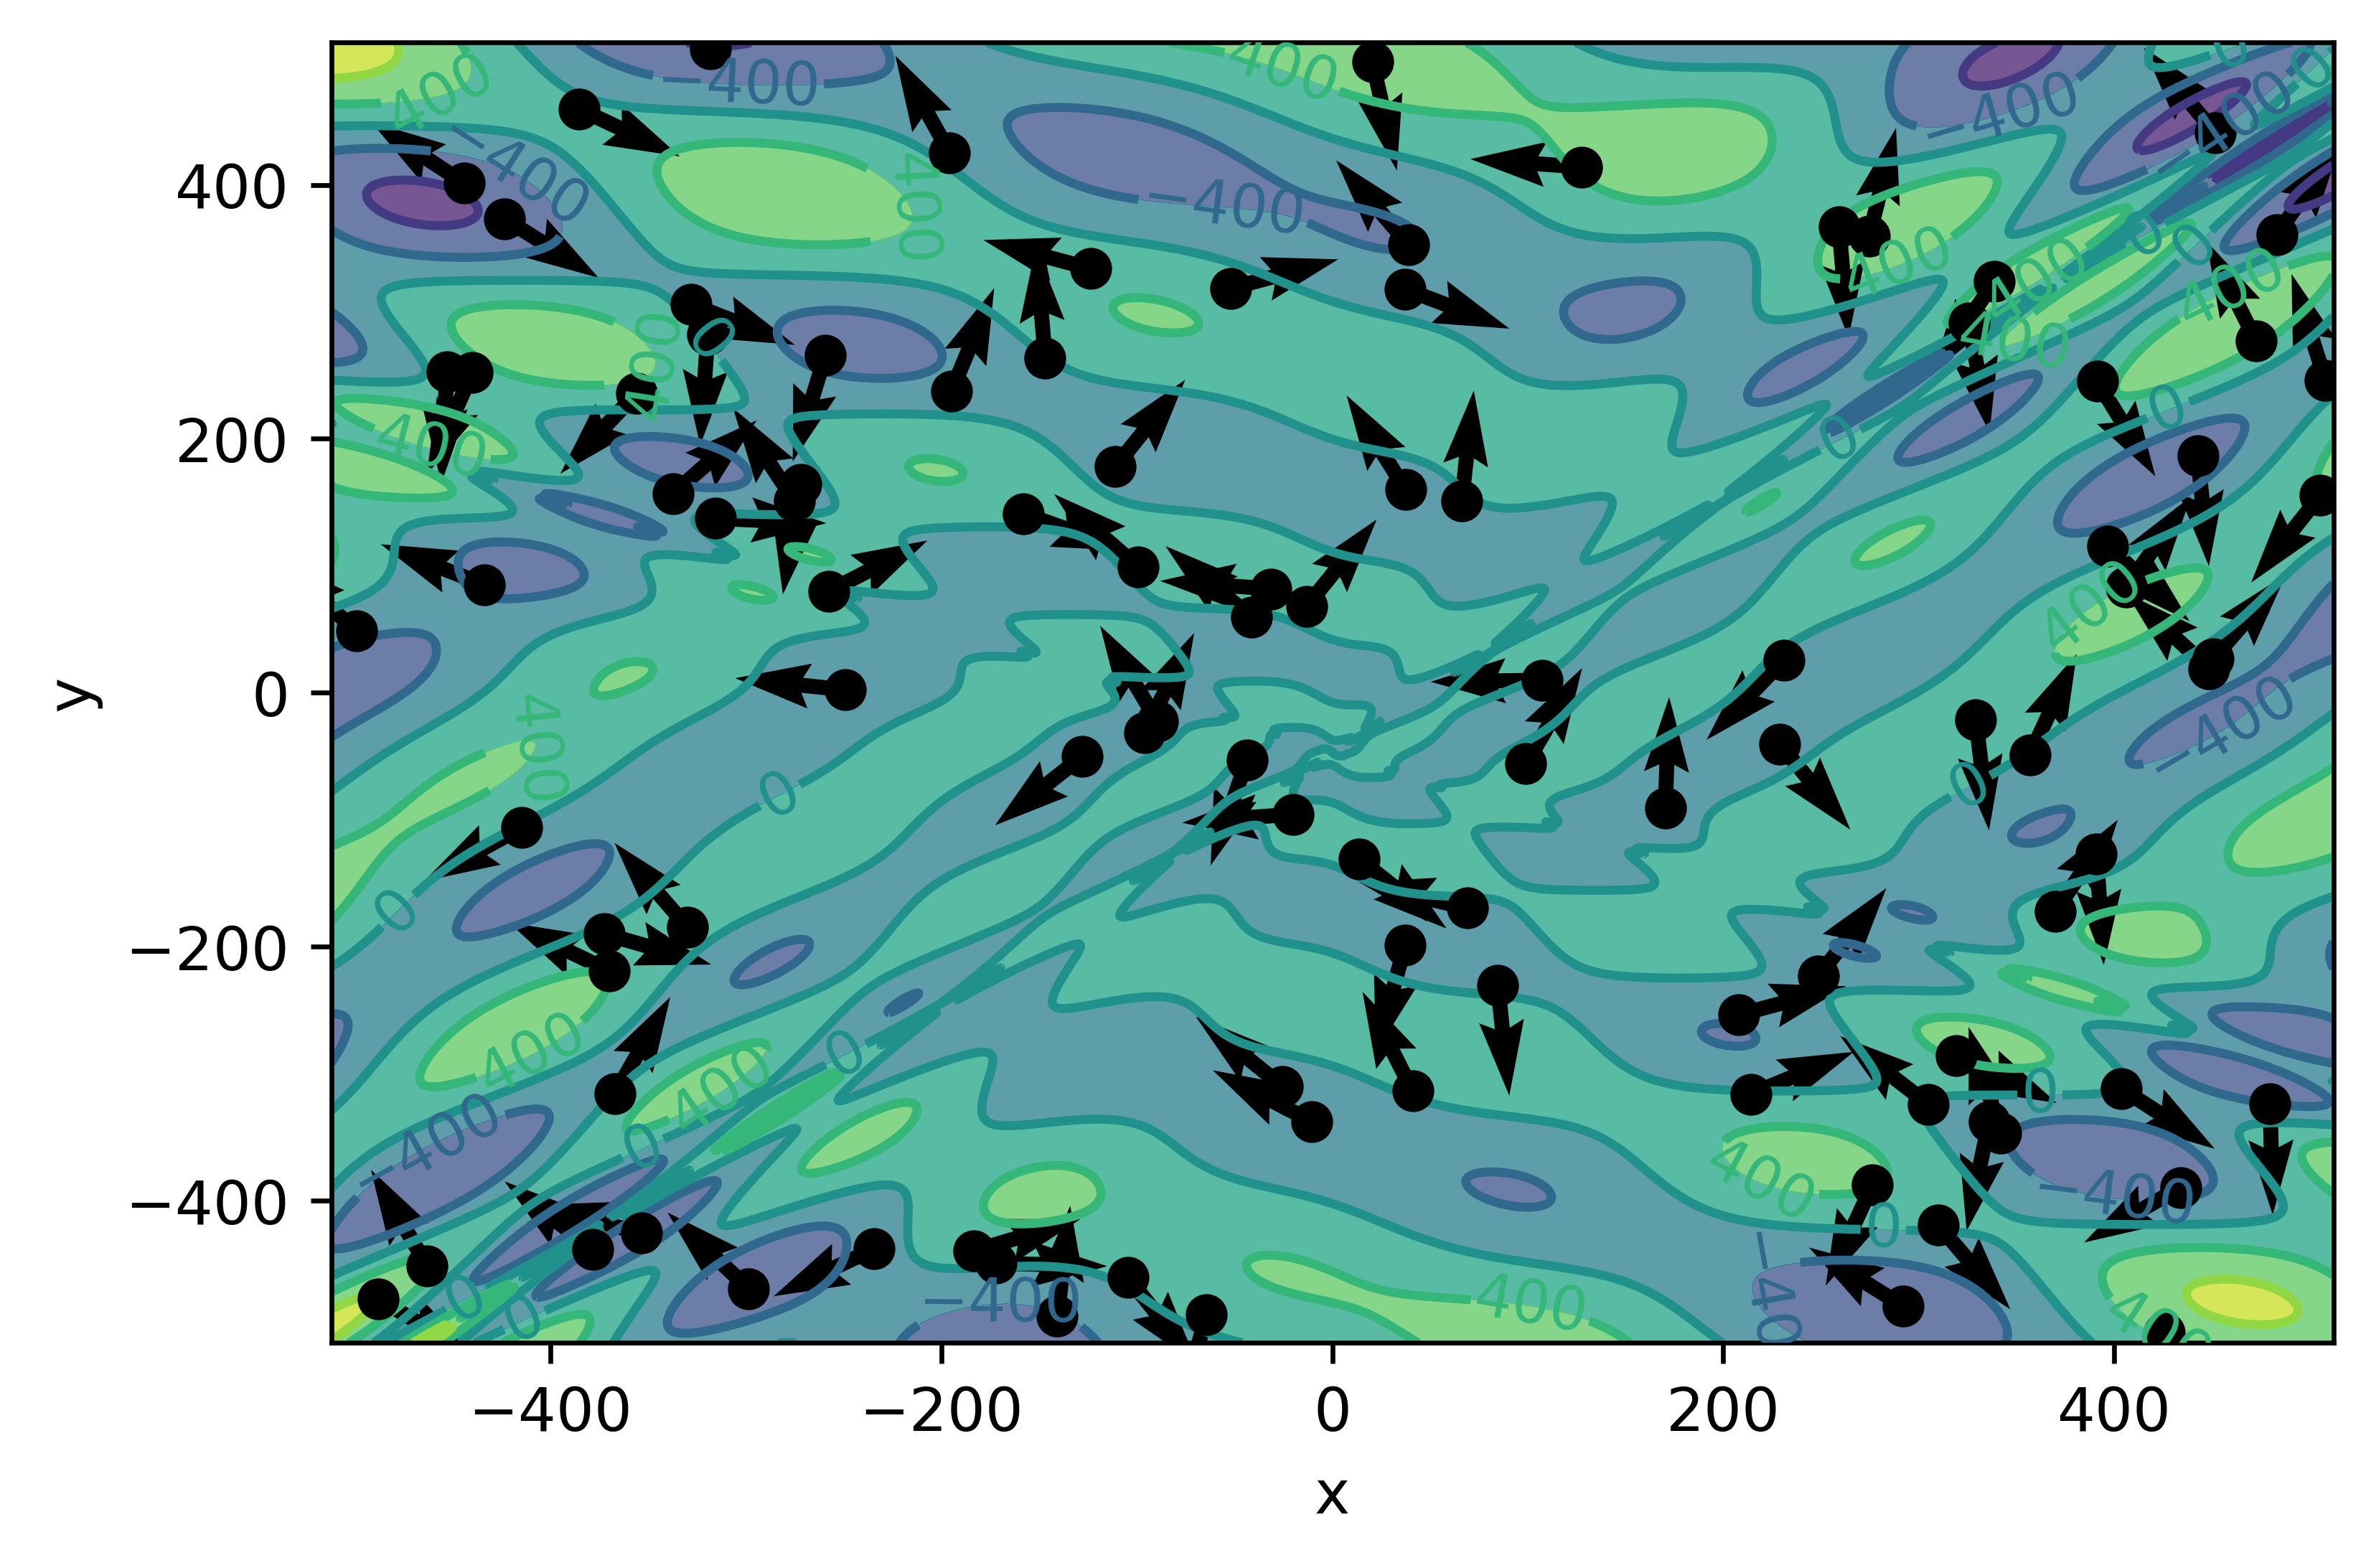
\includegraphics[width=0.5\columnwidth]{figures/ite0.png}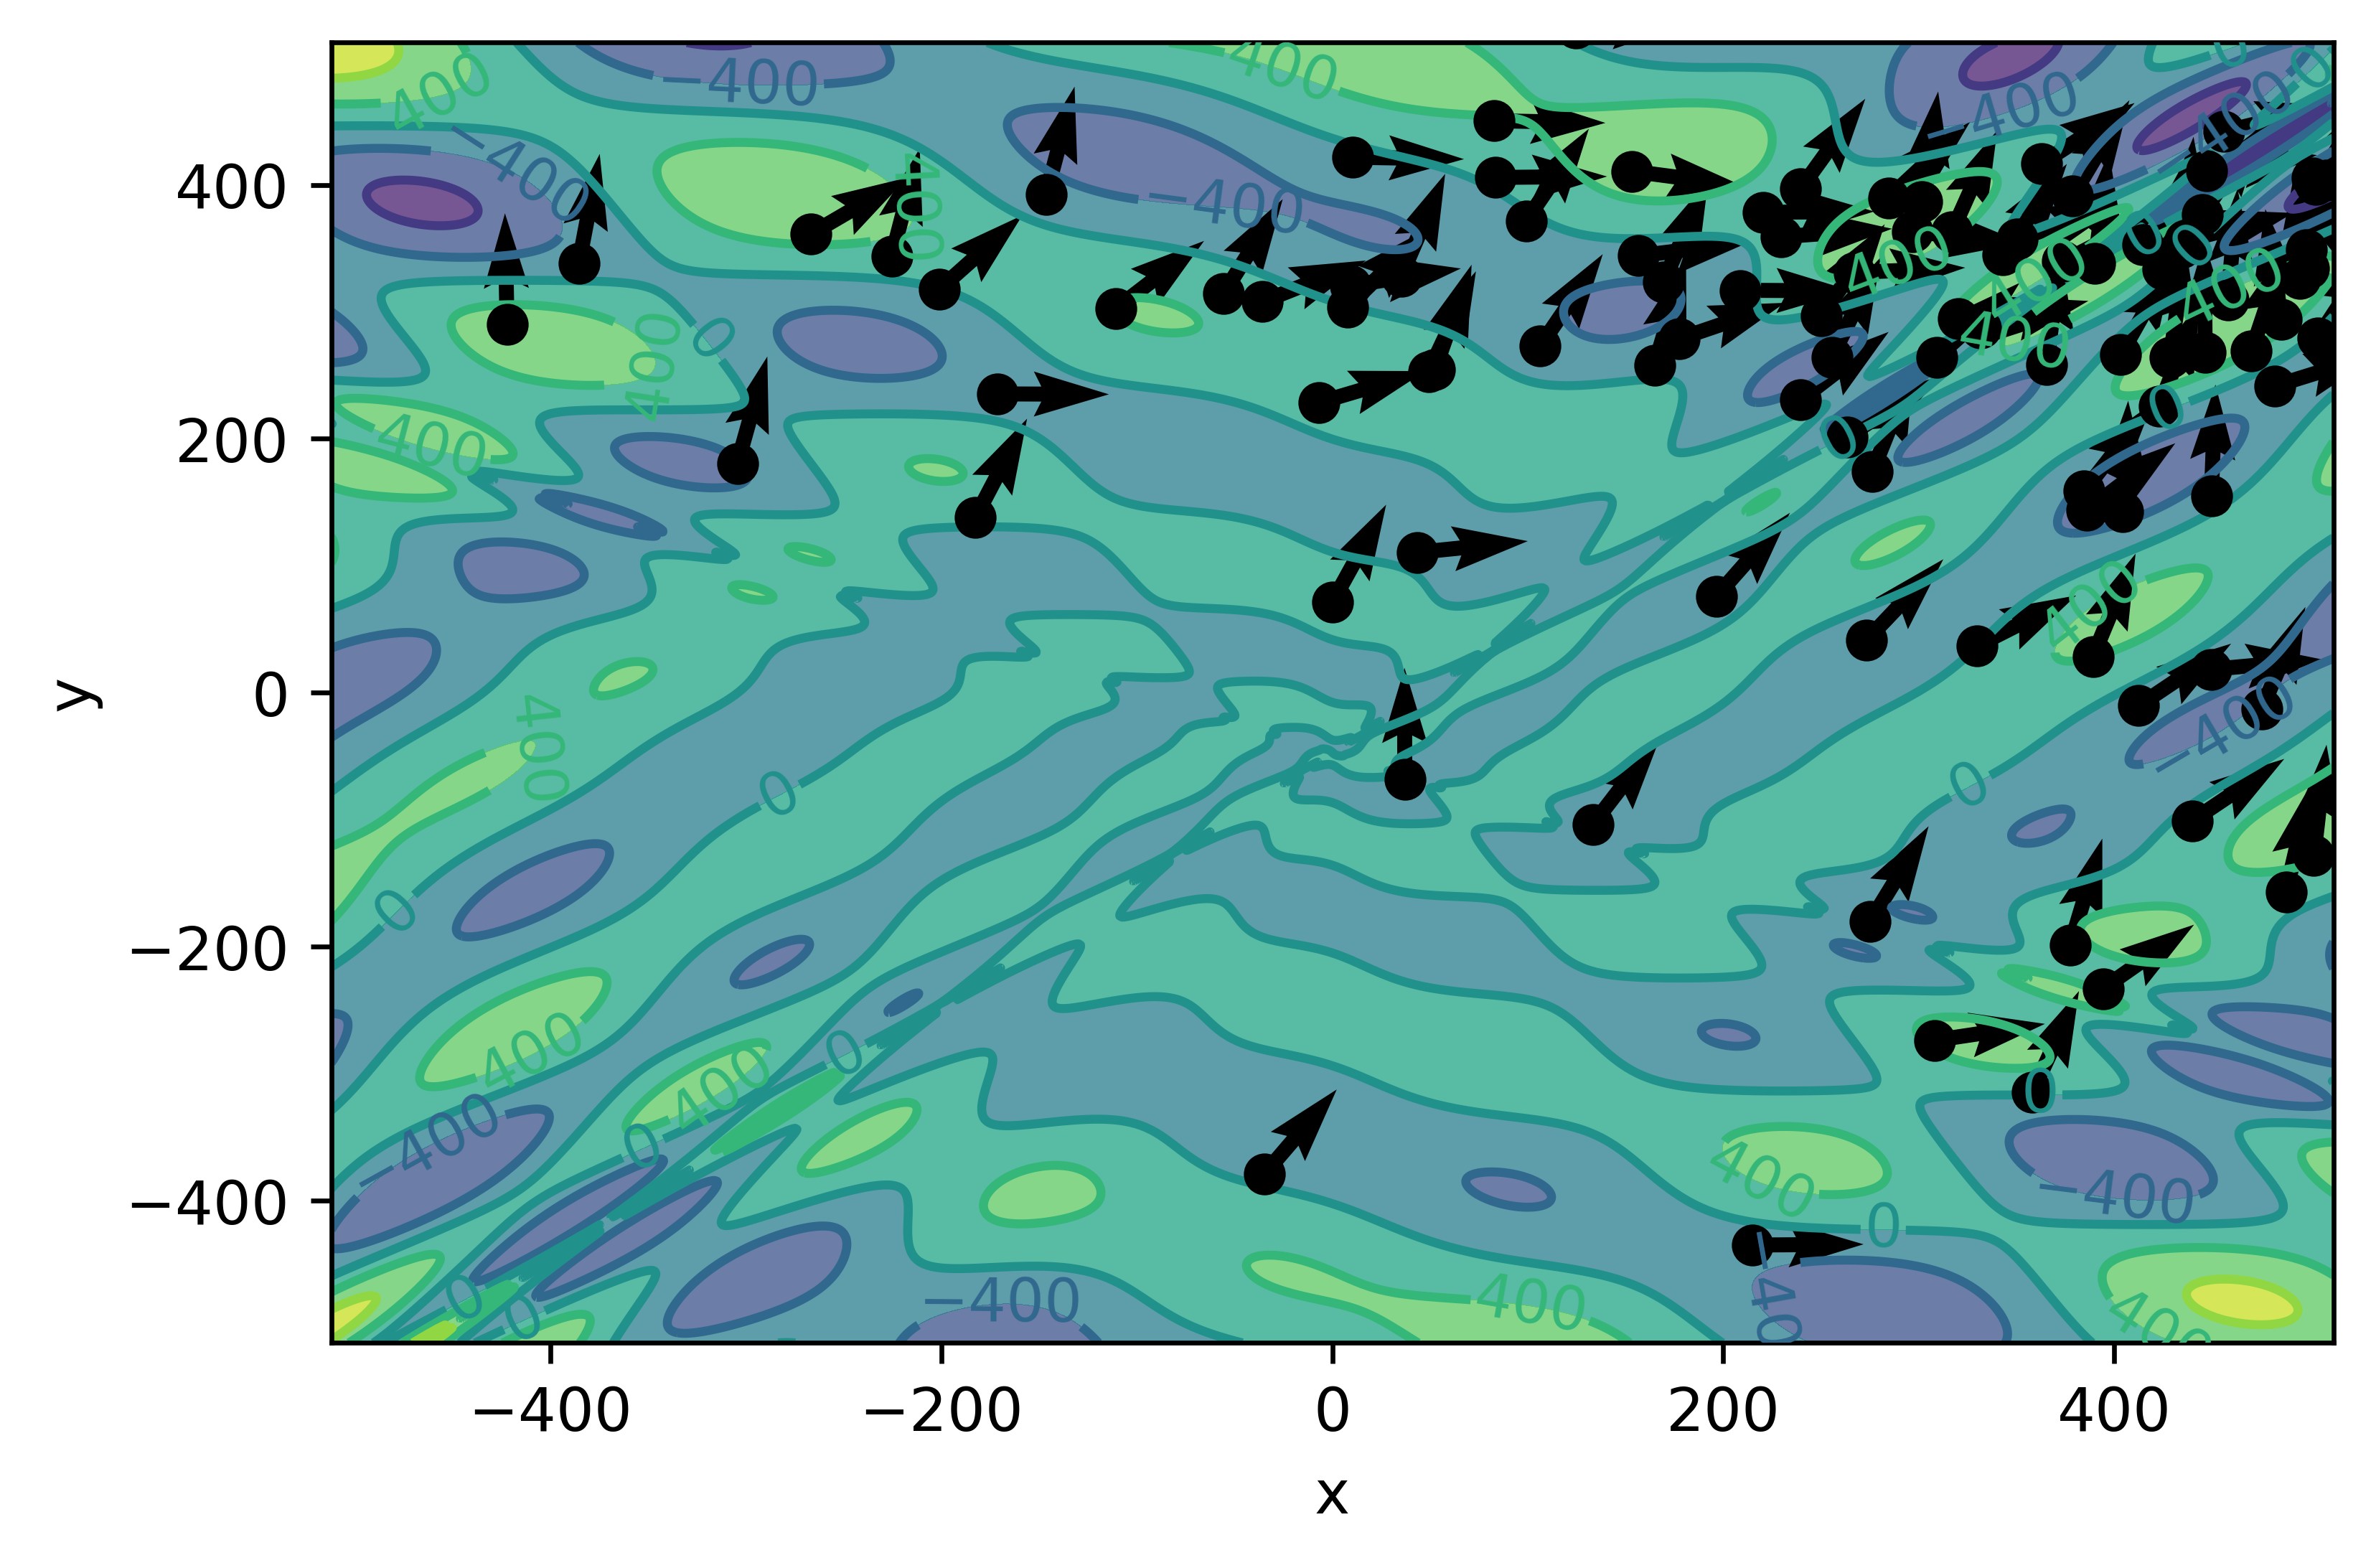
\includegraphics[width=0.5\columnwidth]{figures/ite1.png}
\captionof{figure}{Visualization of particles at initial generation (left) and after one iteration (right)}\medskip
Using only one PSO iteration, particles quickly moved to the \verb+gbest+ area, and allowed some further discoveries, as visible in Figure 4:
\bigskip

\noindent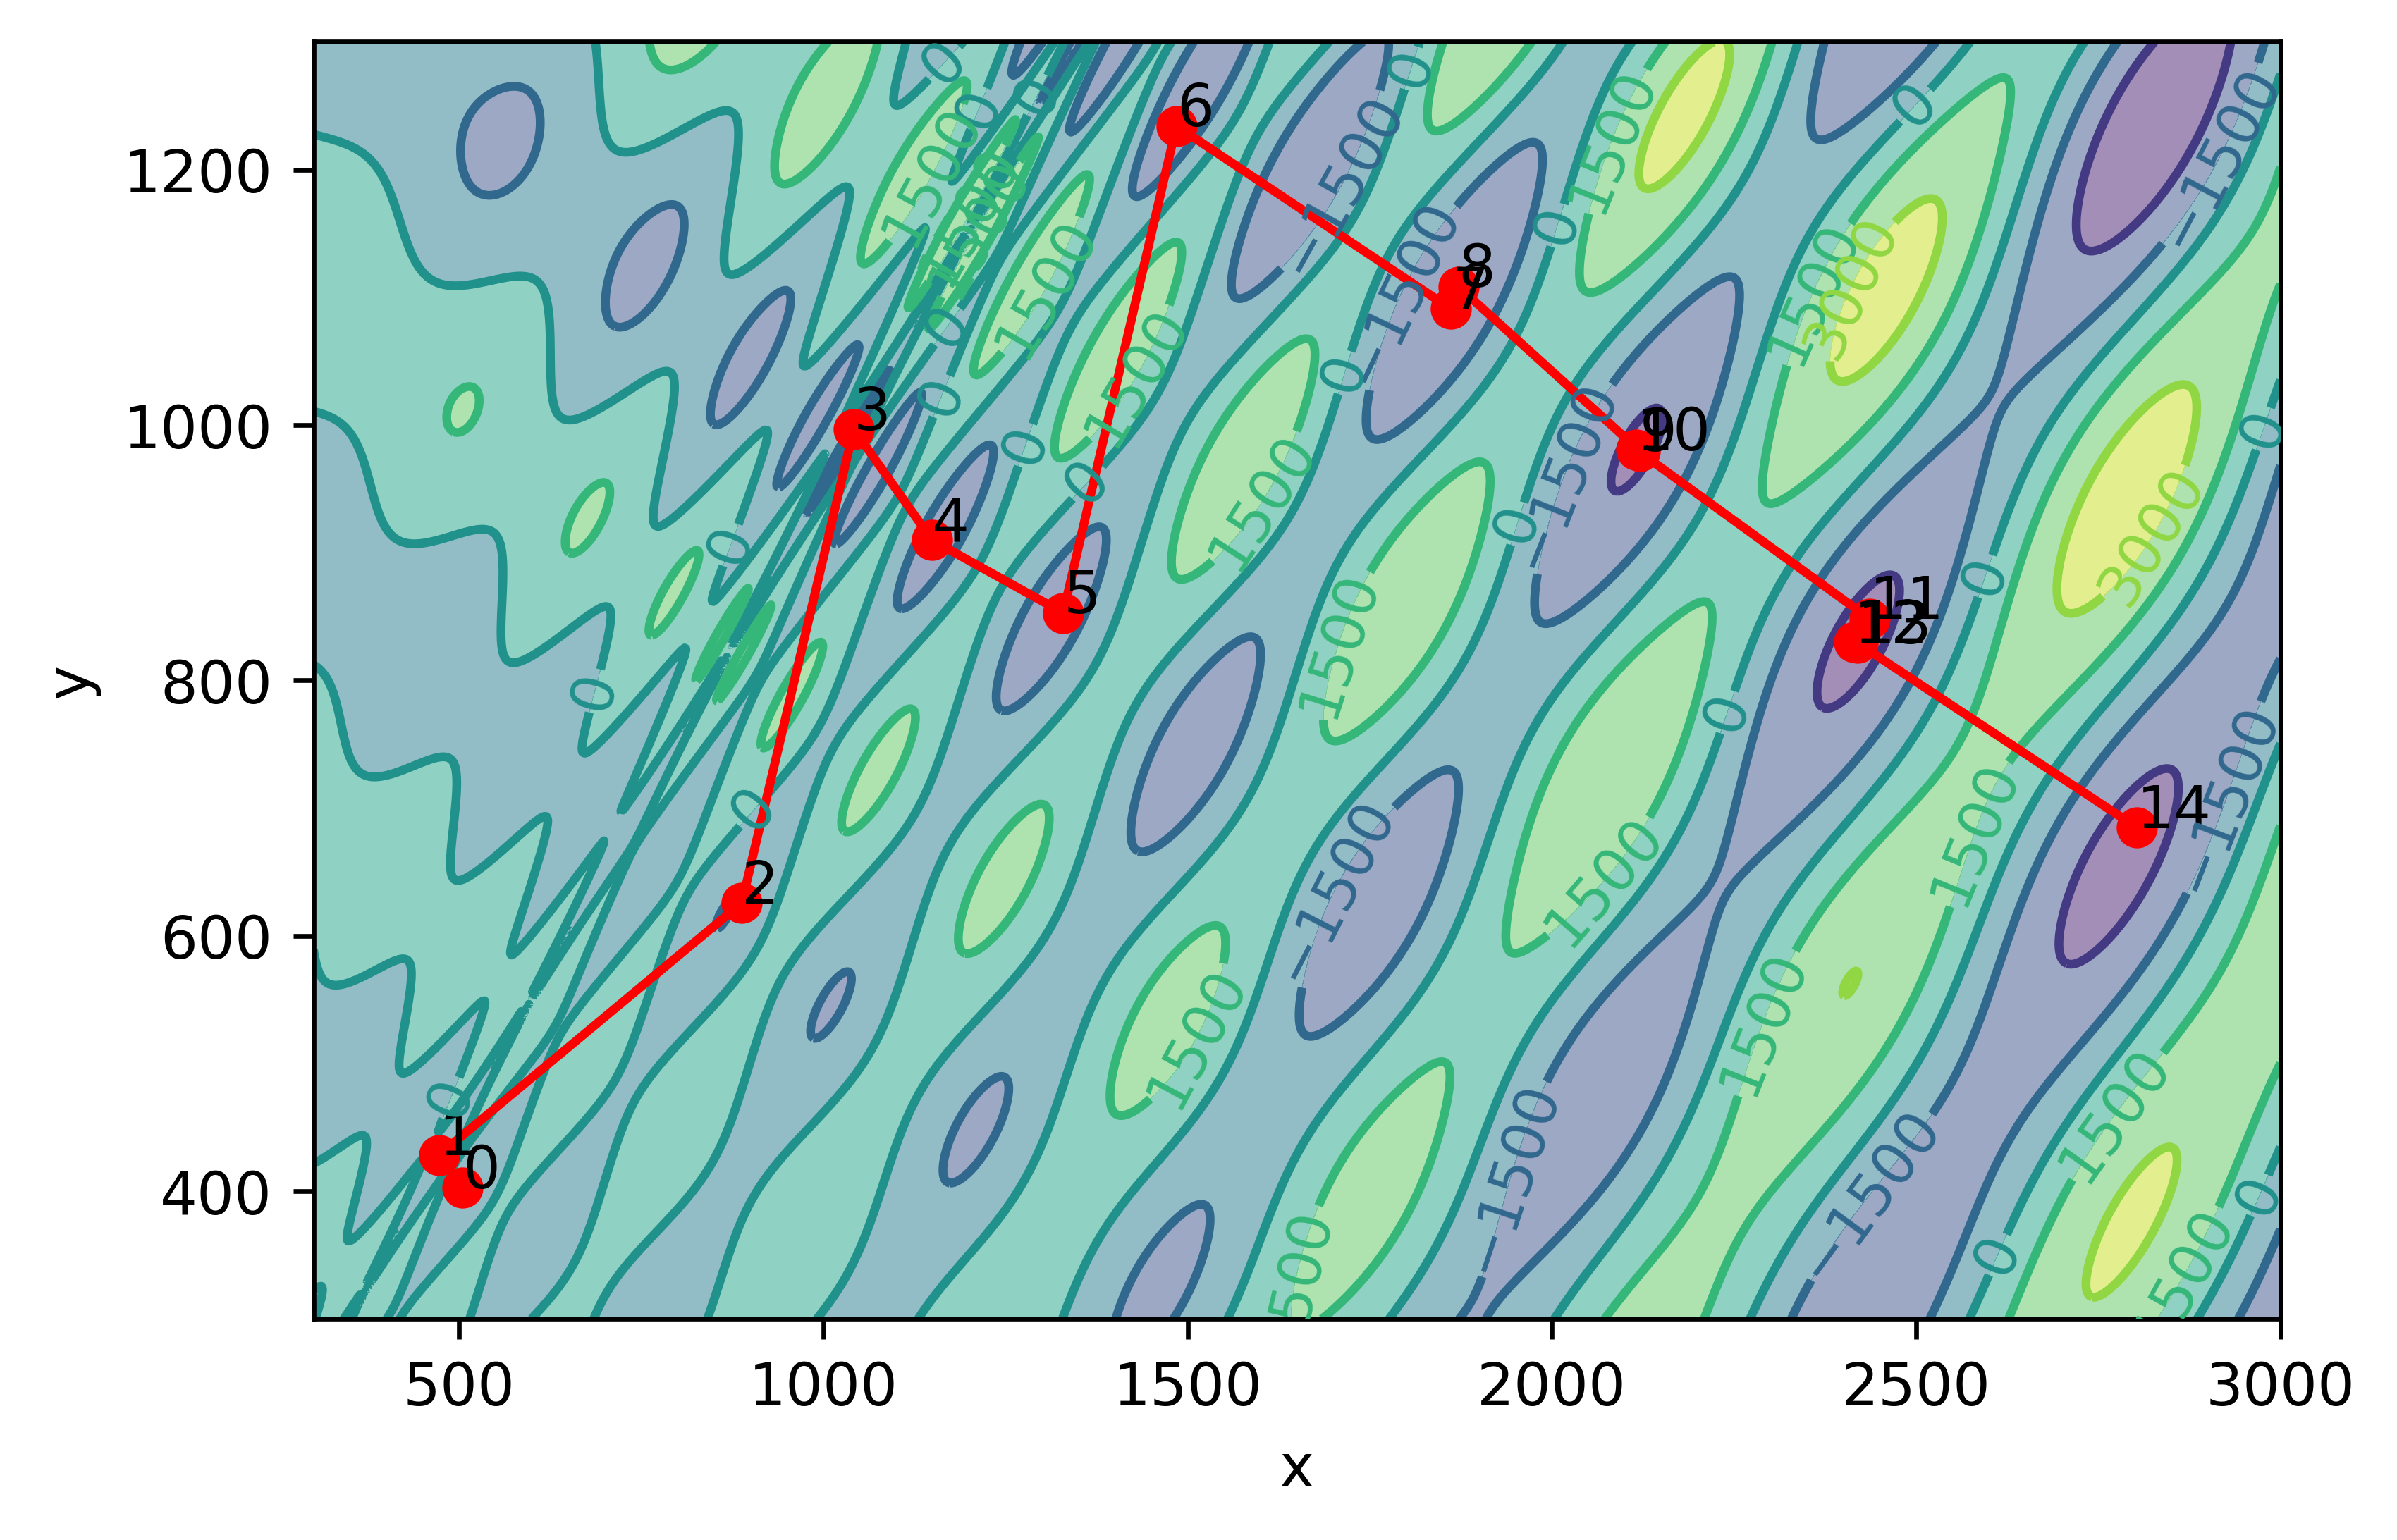
\includegraphics[width=\columnwidth]{figures/eggholder.png} \captionof{figure}{Displacement of global best minimum in the first iterations using the Eggholder function}\medskip 
In this example, the global best minimum managed to move from a basin to another without any problem, even though the spatial steps that separate every minimum are important. It becomes also clear that the more particles are considered, the easier it will be to find new global best minima, although it comes at the cost of more computational time: a compromise needs to be found to allow sufficient sampling.
\section*{Obtained results and comparison to other methods}
Indeed, this method surely seems very advantageous to others when facing unknown crystal phases determination: in the considered planets (Uranus and Neptune), layers of the inner mantle are mainly composed of methane, ammonium and ice water, and are subject to pressure going from 0.1 to 2.5 Mbar \cite{https://doi.org/10.1029/JB085iB01p00225}. However, as they ammonia and water can form hydrogen-bonded networks when they are brought closer in some circumstances, it is possible to see the formation of new phases, lowered in energy.\\
In this case, only mixtures of ammonia and water were studied, and multiple stoechiometric factors were tested, which are all supposedly possible to be observed in those planet's layers. At first, 16 formula units of $( \mathrm{H}_2\mathrm{O})_{X}(\mathrm{N}\mathrm{H}_3)_{Y}$ were tried, however it was soon reduced to only four stable mixtures: ammonia monohydrate (AMH), ammonia dihydrate (ADH), ammonia hemihydrate (AHH), and ammonia quarterhydrate (AQH). The three first configurations are present on our planet at low pressures, making them easy options to consider for stable configurations. However, the last mixture turned out to present some stable crystalline phases at high pressures.\vspace{1em}

Particle Swarn Optimization that was lead on the already-known ammonia hydrates still allowed to make some new discoveries: some phases that were not present in some previously determined phase diagram are actually valid candidates for some pressures: it is the case, for instance, for AMH, with both $P4_3$ and $P2_1/m$ structures that did not appear in the litterature: using PSO in those high-pressure phase evolution studies thus allowed to discover a better stability of the crystal, before changing to the ionic phase $(\mathrm{OH}^-)(\mathrm{NH}_4^+)$. A richer phase diagram was also found for ADH, with phases being stable up to around 100 GPa. These new phases are expected due to the facilitated proton transfer that can occur in the system with the high pressure (in all mixtures): the energy of the system decreases, makes it possible to consider these phases. With usual sampling techniques (such as MD, used in the cited article), finding such phases would be a lot harder, and would require the scientist to know what to look for.\vspace{1em}

Moreover, using PSO also made it possible to discover the stability of another ammonia-water mixture: ammonia quarterhydrate (AQH). Other proportions systematically lead to the dissociation into the previously listed phases, or the basic constituents. This phases begins to exist at already high pressures (starting from 8.5 GPa), and decomposes back into ices again around 300 GPa.

\end{multicols}
\begin{figure}[h]
    \centering
    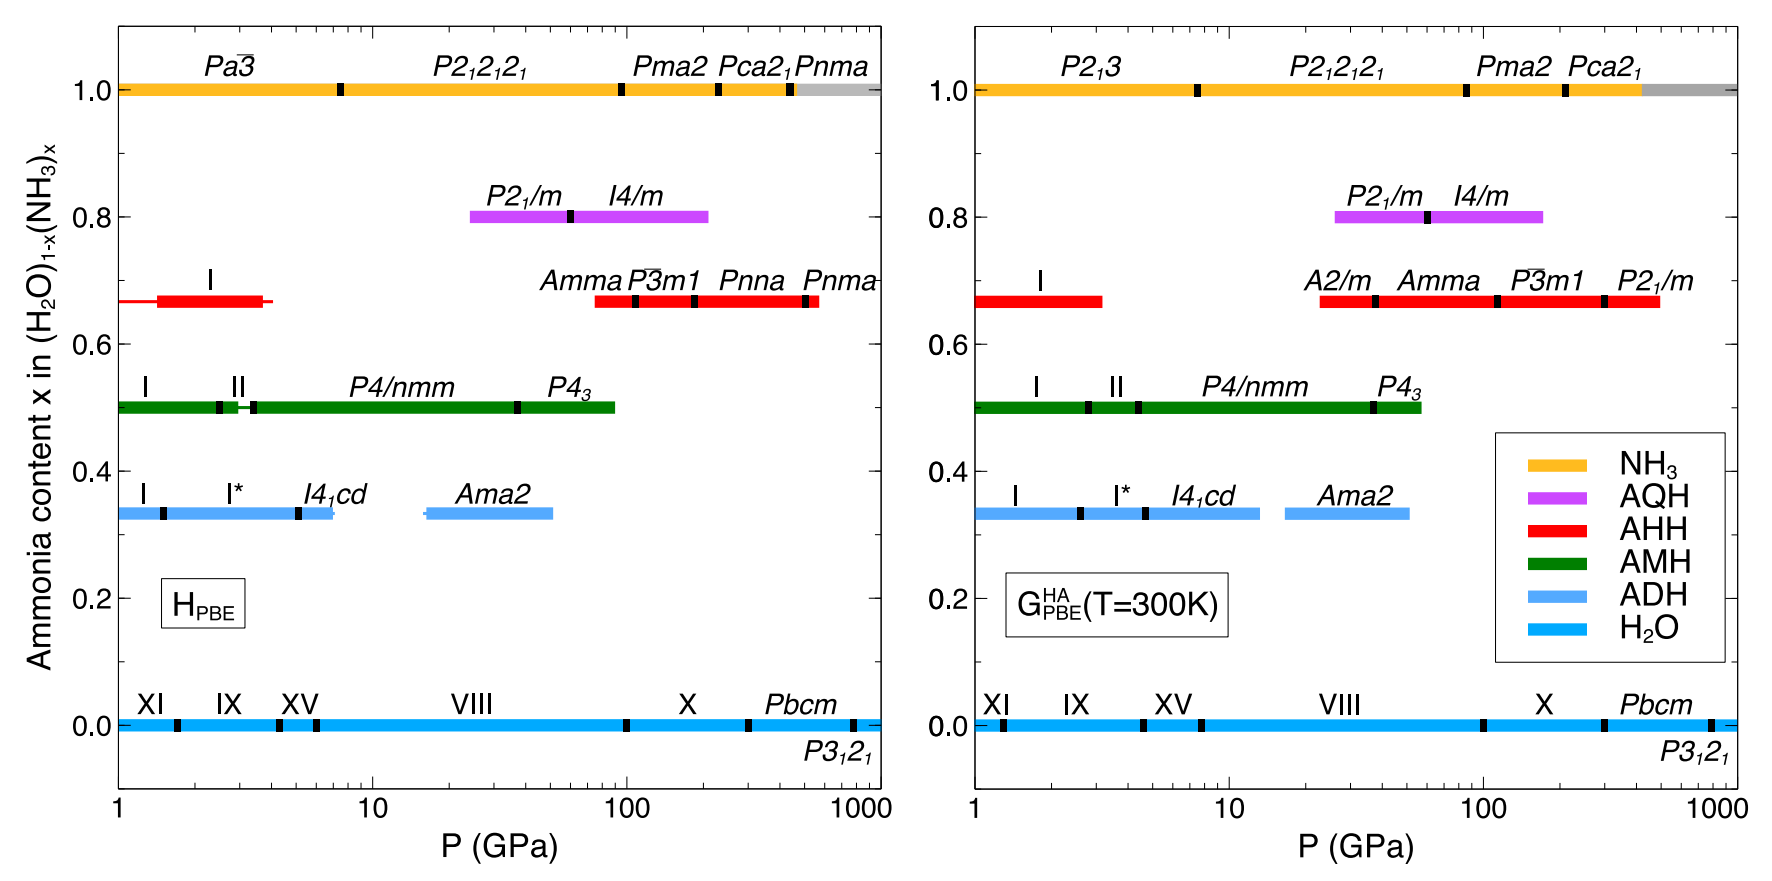
\includegraphics[width=\textwidth]{figures/phase-diagram.png}
    \caption{Phase stability ranges for binary ammonia-water mixtures as a function of pressure, for the ground state (left) and at T = 300 K (right), by Naden Robinson et al. \cite{original}}
\end{figure}
\begin{multicols}{2}

\section*{Conclusion}
As a matter of conclusion, blabla\\et puis reblabla
\end{multicols}
\bibliographystyle{bibstyle.bst}
\bibliography{articles}

\end{document}